% Created 2024-05-27 Mon 08:21
% Intended LaTeX compiler: pdflatex
\documentclass[11pt]{article}
\usepackage[utf8]{inputenc}
\usepackage[T1]{fontenc}
\usepackage{graphicx}
\usepackage{longtable}
\usepackage{wrapfig}
\usepackage{rotating}
\usepackage[normalem]{ulem}
\usepackage{amsmath}
\usepackage{amssymb}
\usepackage{capt-of}
\usepackage{hyperref}
\usepackage{minted}
\usepackage[russian]{babel}
\author{cofeek-codes}
\date{\today}
\title{AJAX}
\hypersetup{
 pdfauthor={cofeek-codes},
 pdftitle={AJAX},
 pdfkeywords={},
 pdfsubject={},
 pdfcreator={Emacs 28.2 (Org mode 9.5.5)}, 
 pdflang={Russian}}
\begin{document}

\maketitle
\tableofcontents


\section{AJAX}
\label{sec:orga5f6d96}

\textbf{AJAX (Asynchronous Javascript and XML)} - технология для взаимодействия с сервером без перезагрузки страниц

\begin{center}
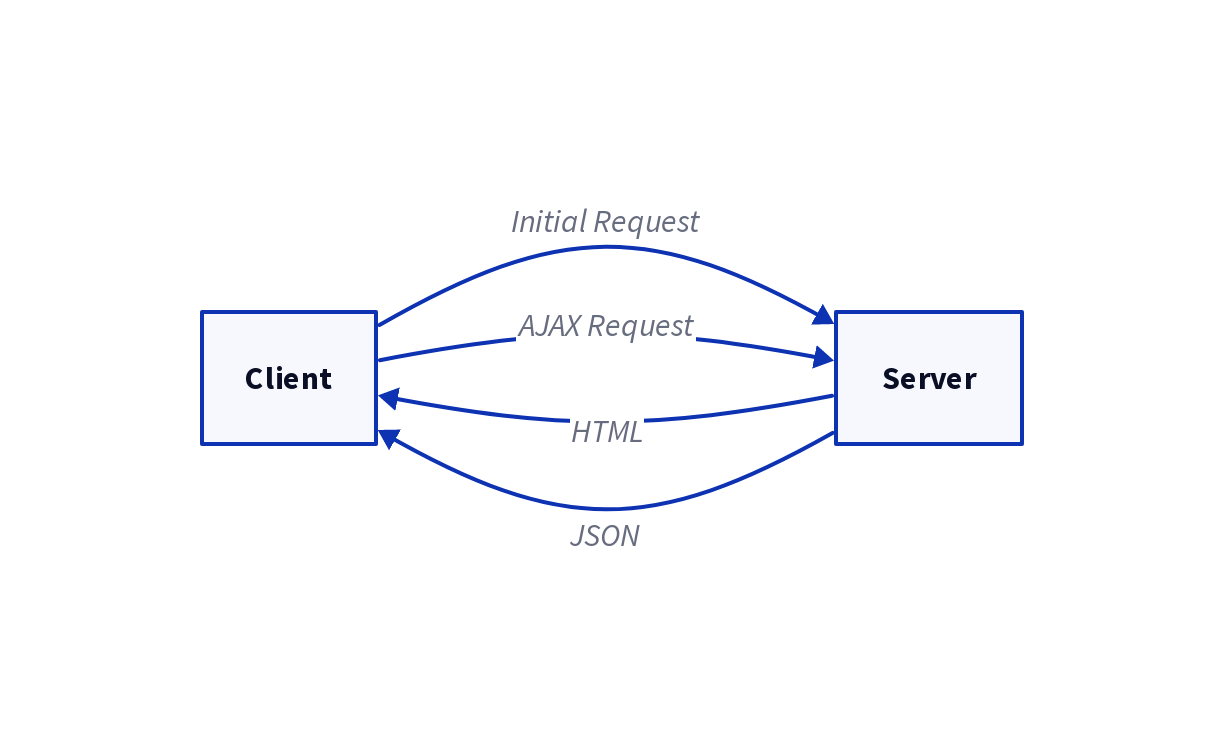
\includegraphics[width=.9\linewidth]{./schema.png}
\end{center}

\subsection{Что использует}
\label{sec:org658e1e9}

\begin{itemize}
\item (X)HTML, CSS
\item DOM-модель и js-операции на стороне клиента для динамики
\item XMLHttpRequest для асинхронного взаимодействия с сервером
\item JSON часто используется для обмена данными (могут быть и другие форматы)
\end{itemize}

\subsection{Сферы применения}
\label{sec:org0e70e0a}

\begin{enumerate}
\item Небольшие элементы с элементарными действиями (подписаться, загрузить, оценить)
\item Динамическая подгрузка данных с сервера
\item Незаметные (для пользователя) действия
\item Непрерывная подгрузка информации с сервера (чаты)
\item Автодополнение в поисковых движках
\end{enumerate}
\end{document}